% ===== regularization =====
\section*{Regularization}

\subsection*{What Regularization Does}

Take the linear regression loss and add one extra term:
\[
\underbrace{\tfrac{1}{2}\|\mathbf{t} - X\mathbf{w}\|^2}_{\text{linear regression}}
\;+\;
\underbrace{\tfrac{\lambda}{2}\|\mathbf{w}\|^2}_{\text{keep weights small}}
\]
The first term is just linear regression. The second term (the \textbf{regularization term}) is an incentive to keep the weights small. $\lambda$ sets how much it matters: the bigger $\lambda$, the harder big weights are penalized.

\begin{keeptogether}
\textbf{Example.} Fit a degree-7 polynomial to the 8 points from Overfitting vs.\ Underfitting, with three values of $\lambda$:

{\centering
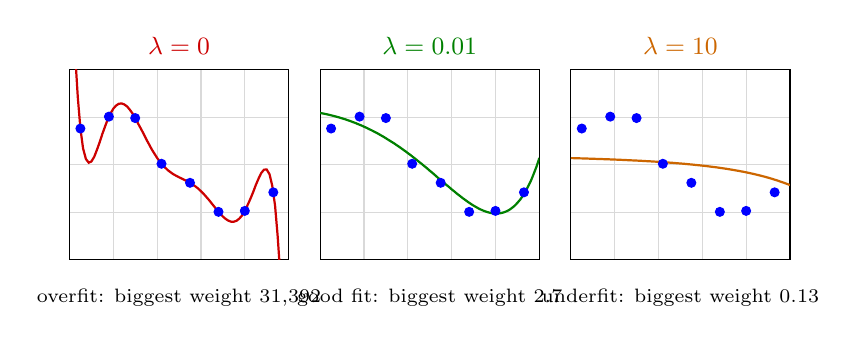
\begin{tikzpicture}
\begin{axis}[name=p0,
    width=0.36\linewidth, height=4cm,
    xmin=0, xmax=1, ymin=-2, ymax=2, enlargelimits=false,
    grid=major, grid style={gray!30}, major tick length=0pt,
    xticklabels={}, yticklabels={},
    title={\small\textbf{$\lambda = 0$}}, title style={text=red!80!black, yshift=-4pt},
    xlabel={\scriptsize overfit: biggest weight $31{,}392$}, label style={font=\scriptsize}]
\addplot[only marks, mark=*, blue, mark size=1.6pt] coordinates {(0.05,0.76) (0.18,1.01) (0.3,0.98) (0.42,0.02) (0.55,-0.38) (0.68,-0.99) (0.8,-0.97) (0.93,-0.58)};
\addplot[thick, red!80!black] coordinates {(0.000,2.400) (0.013,2.400) (0.025,2.396) (0.038,1.422) (0.050,0.760) (0.062,0.345) (0.075,0.121) (0.088,0.042) (0.100,0.068) (0.113,0.166) (0.125,0.308) (0.138,0.474) (0.150,0.646) (0.163,0.810) (0.175,0.957) (0.188,1.081) (0.200,1.177) (0.213,1.244) (0.225,1.280) (0.238,1.287) (0.250,1.267) (0.263,1.223) (0.275,1.158) (0.288,1.075) (0.300,0.980) (0.312,0.875) (0.325,0.765) (0.338,0.652) (0.350,0.539) (0.363,0.430) (0.375,0.326) (0.388,0.230) (0.400,0.142) (0.413,0.063) (0.425,-0.007) (0.438,-0.067) (0.450,-0.119) (0.463,-0.164) (0.475,-0.202) (0.488,-0.235) (0.500,-0.264) (0.513,-0.292) (0.525,-0.319) (0.537,-0.348) (0.550,-0.380) (0.562,-0.416) (0.575,-0.457) (0.588,-0.504) (0.600,-0.557) (0.613,-0.616) (0.625,-0.680) (0.638,-0.748) (0.650,-0.819) (0.663,-0.892) (0.675,-0.963) (0.688,-1.029) (0.700,-1.089) (0.713,-1.139) (0.725,-1.176) (0.738,-1.196) (0.750,-1.197) (0.763,-1.176) (0.775,-1.131) (0.788,-1.063) (0.800,-0.970) (0.812,-0.855) (0.825,-0.722) (0.838,-0.577) (0.850,-0.429) (0.863,-0.289) (0.875,-0.174) (0.888,-0.103) (0.900,-0.102) (0.913,-0.202) (0.925,-0.438) (0.938,-0.855) (0.950,-1.504) (0.963,-2.400) (0.975,-2.400) (0.988,-2.400) (1.000,-2.400)};
\end{axis}
\begin{axis}[name=p1, at={(p0.east)}, anchor=west, xshift=0.4cm,
    width=0.36\linewidth, height=4cm,
    xmin=0, xmax=1, ymin=-2, ymax=2, enlargelimits=false,
    grid=major, grid style={gray!30}, major tick length=0pt,
    xticklabels={}, yticklabels={},
    title={\small\textbf{$\lambda = 0.01$}}, title style={text=green!50!black, yshift=-4pt},
    xlabel={\scriptsize good fit: biggest weight $2.7$}, label style={font=\scriptsize}]
\addplot[only marks, mark=*, blue, mark size=1.6pt] coordinates {(0.05,0.76) (0.18,1.01) (0.3,0.98) (0.42,0.02) (0.55,-0.38) (0.68,-0.99) (0.8,-0.97) (0.93,-0.58)};
\addplot[thick, green!50!black] coordinates {(0.000,1.087) (0.013,1.076) (0.025,1.065) (0.038,1.052) (0.050,1.038) (0.062,1.024) (0.075,1.008) (0.088,0.992) (0.100,0.974) (0.113,0.956) (0.125,0.937) (0.138,0.916) (0.150,0.895) (0.163,0.873) (0.175,0.849) (0.188,0.825) (0.200,0.799) (0.213,0.773) (0.225,0.745) (0.238,0.716) (0.250,0.687) (0.263,0.656) (0.275,0.624) (0.288,0.590) (0.300,0.556) (0.312,0.521) (0.325,0.484) (0.338,0.447) (0.350,0.408) (0.363,0.369) (0.375,0.328) (0.388,0.287) (0.400,0.244) (0.413,0.201) (0.425,0.157) (0.438,0.111) (0.450,0.065) (0.463,0.019) (0.475,-0.028) (0.488,-0.076) (0.500,-0.125) (0.513,-0.173) (0.525,-0.222) (0.537,-0.272) (0.550,-0.321) (0.562,-0.370) (0.575,-0.419) (0.588,-0.468) (0.600,-0.516) (0.613,-0.564) (0.625,-0.611) (0.638,-0.656) (0.650,-0.700) (0.663,-0.743) (0.675,-0.784) (0.688,-0.823) (0.700,-0.859) (0.713,-0.893) (0.725,-0.924) (0.738,-0.952) (0.750,-0.975) (0.763,-0.995) (0.775,-1.010) (0.788,-1.020) (0.800,-1.025) (0.812,-1.024) (0.825,-1.016) (0.838,-1.001) (0.850,-0.979) (0.863,-0.949) (0.875,-0.909) (0.888,-0.860) (0.900,-0.801) (0.913,-0.731) (0.925,-0.649) (0.938,-0.554) (0.950,-0.446) (0.963,-0.323) (0.975,-0.185) (0.988,-0.031) (1.000,0.141)};
\end{axis}
\begin{axis}[name=p2, at={(p1.east)}, anchor=west, xshift=0.4cm,
    width=0.36\linewidth, height=4cm,
    xmin=0, xmax=1, ymin=-2, ymax=2, enlargelimits=false,
    grid=major, grid style={gray!30}, major tick length=0pt,
    xticklabels={}, yticklabels={},
    title={\small\textbf{$\lambda = 10$}}, title style={text=orange!80!black, yshift=-4pt},
    xlabel={\scriptsize underfit: biggest weight $0.13$}, label style={font=\scriptsize}]
\addplot[only marks, mark=*, blue, mark size=1.6pt] coordinates {(0.05,0.76) (0.18,1.01) (0.3,0.98) (0.42,0.02) (0.55,-0.38) (0.68,-0.99) (0.8,-0.97) (0.93,-0.58)};
\addplot[thick, orange!80!black] coordinates {(0.000,0.139) (0.013,0.138) (0.025,0.136) (0.038,0.134) (0.050,0.133) (0.062,0.131) (0.075,0.129) (0.088,0.127) (0.100,0.125) (0.113,0.123) (0.125,0.121) (0.138,0.119) (0.150,0.117) (0.163,0.115) (0.175,0.113) (0.188,0.110) (0.200,0.108) (0.213,0.106) (0.225,0.103) (0.238,0.101) (0.250,0.098) (0.263,0.095) (0.275,0.092) (0.288,0.090) (0.300,0.087) (0.312,0.084) (0.325,0.081) (0.338,0.077) (0.350,0.074) (0.363,0.071) (0.375,0.067) (0.388,0.064) (0.400,0.060) (0.413,0.056) (0.425,0.052) (0.438,0.048) (0.450,0.044) (0.463,0.040) (0.475,0.035) (0.488,0.030) (0.500,0.026) (0.513,0.021) (0.525,0.016) (0.537,0.010) (0.550,0.005) (0.562,-0.001) (0.575,-0.007) (0.588,-0.013) (0.600,-0.019) (0.613,-0.026) (0.625,-0.032) (0.638,-0.040) (0.650,-0.047) (0.663,-0.054) (0.675,-0.062) (0.688,-0.071) (0.700,-0.079) (0.713,-0.088) (0.725,-0.097) (0.738,-0.107) (0.750,-0.117) (0.763,-0.127) (0.775,-0.138) (0.788,-0.149) (0.800,-0.160) (0.812,-0.172) (0.825,-0.185) (0.838,-0.198) (0.850,-0.212) (0.863,-0.226) (0.875,-0.241) (0.888,-0.256) (0.900,-0.272) (0.913,-0.289) (0.925,-0.307) (0.938,-0.325) (0.950,-0.344) (0.963,-0.364) (0.975,-0.384) (0.988,-0.406) (1.000,-0.428)};
\end{axis}
\end{tikzpicture}
\par}
\end{keeptogether}

\begin{itemize}
  \item \textbf{$\lambda = 0$}: plain linear regression. A high-degree polynomial hits every point by using huge weights that cancel each other out, which is what makes the curve wiggle.
  \item \textbf{$\lambda$ in between}: big weights now cost too much, so the curve can't wiggle. It misses each point a little and follows the real pattern.
  \item \textbf{$\lambda$ too big}: every weight is pushed toward 0, so the curve is almost flat. It underfits.
\end{itemize}

So regularization fixes overfitting by keeping the weights from getting too big.

